\section{Results}

\subsection{Transcriptomics enrichment analysis: Validation of the controls}

When conducting \acrlong{de} analysis, the user has to ensure that controls are separated from the tumours.
Homogeneity among the controls, similarity between the control and tumour counts distribution are also factors that can improve the results.
Despite that the controls should be separated from the tumours, it has been observed for different types of cancer in \acrshort{tcga} that the gene expression follows a similar distribution between both conditions \cite*{Decamps2021}.

\begin{figure}
    \begin{center}
        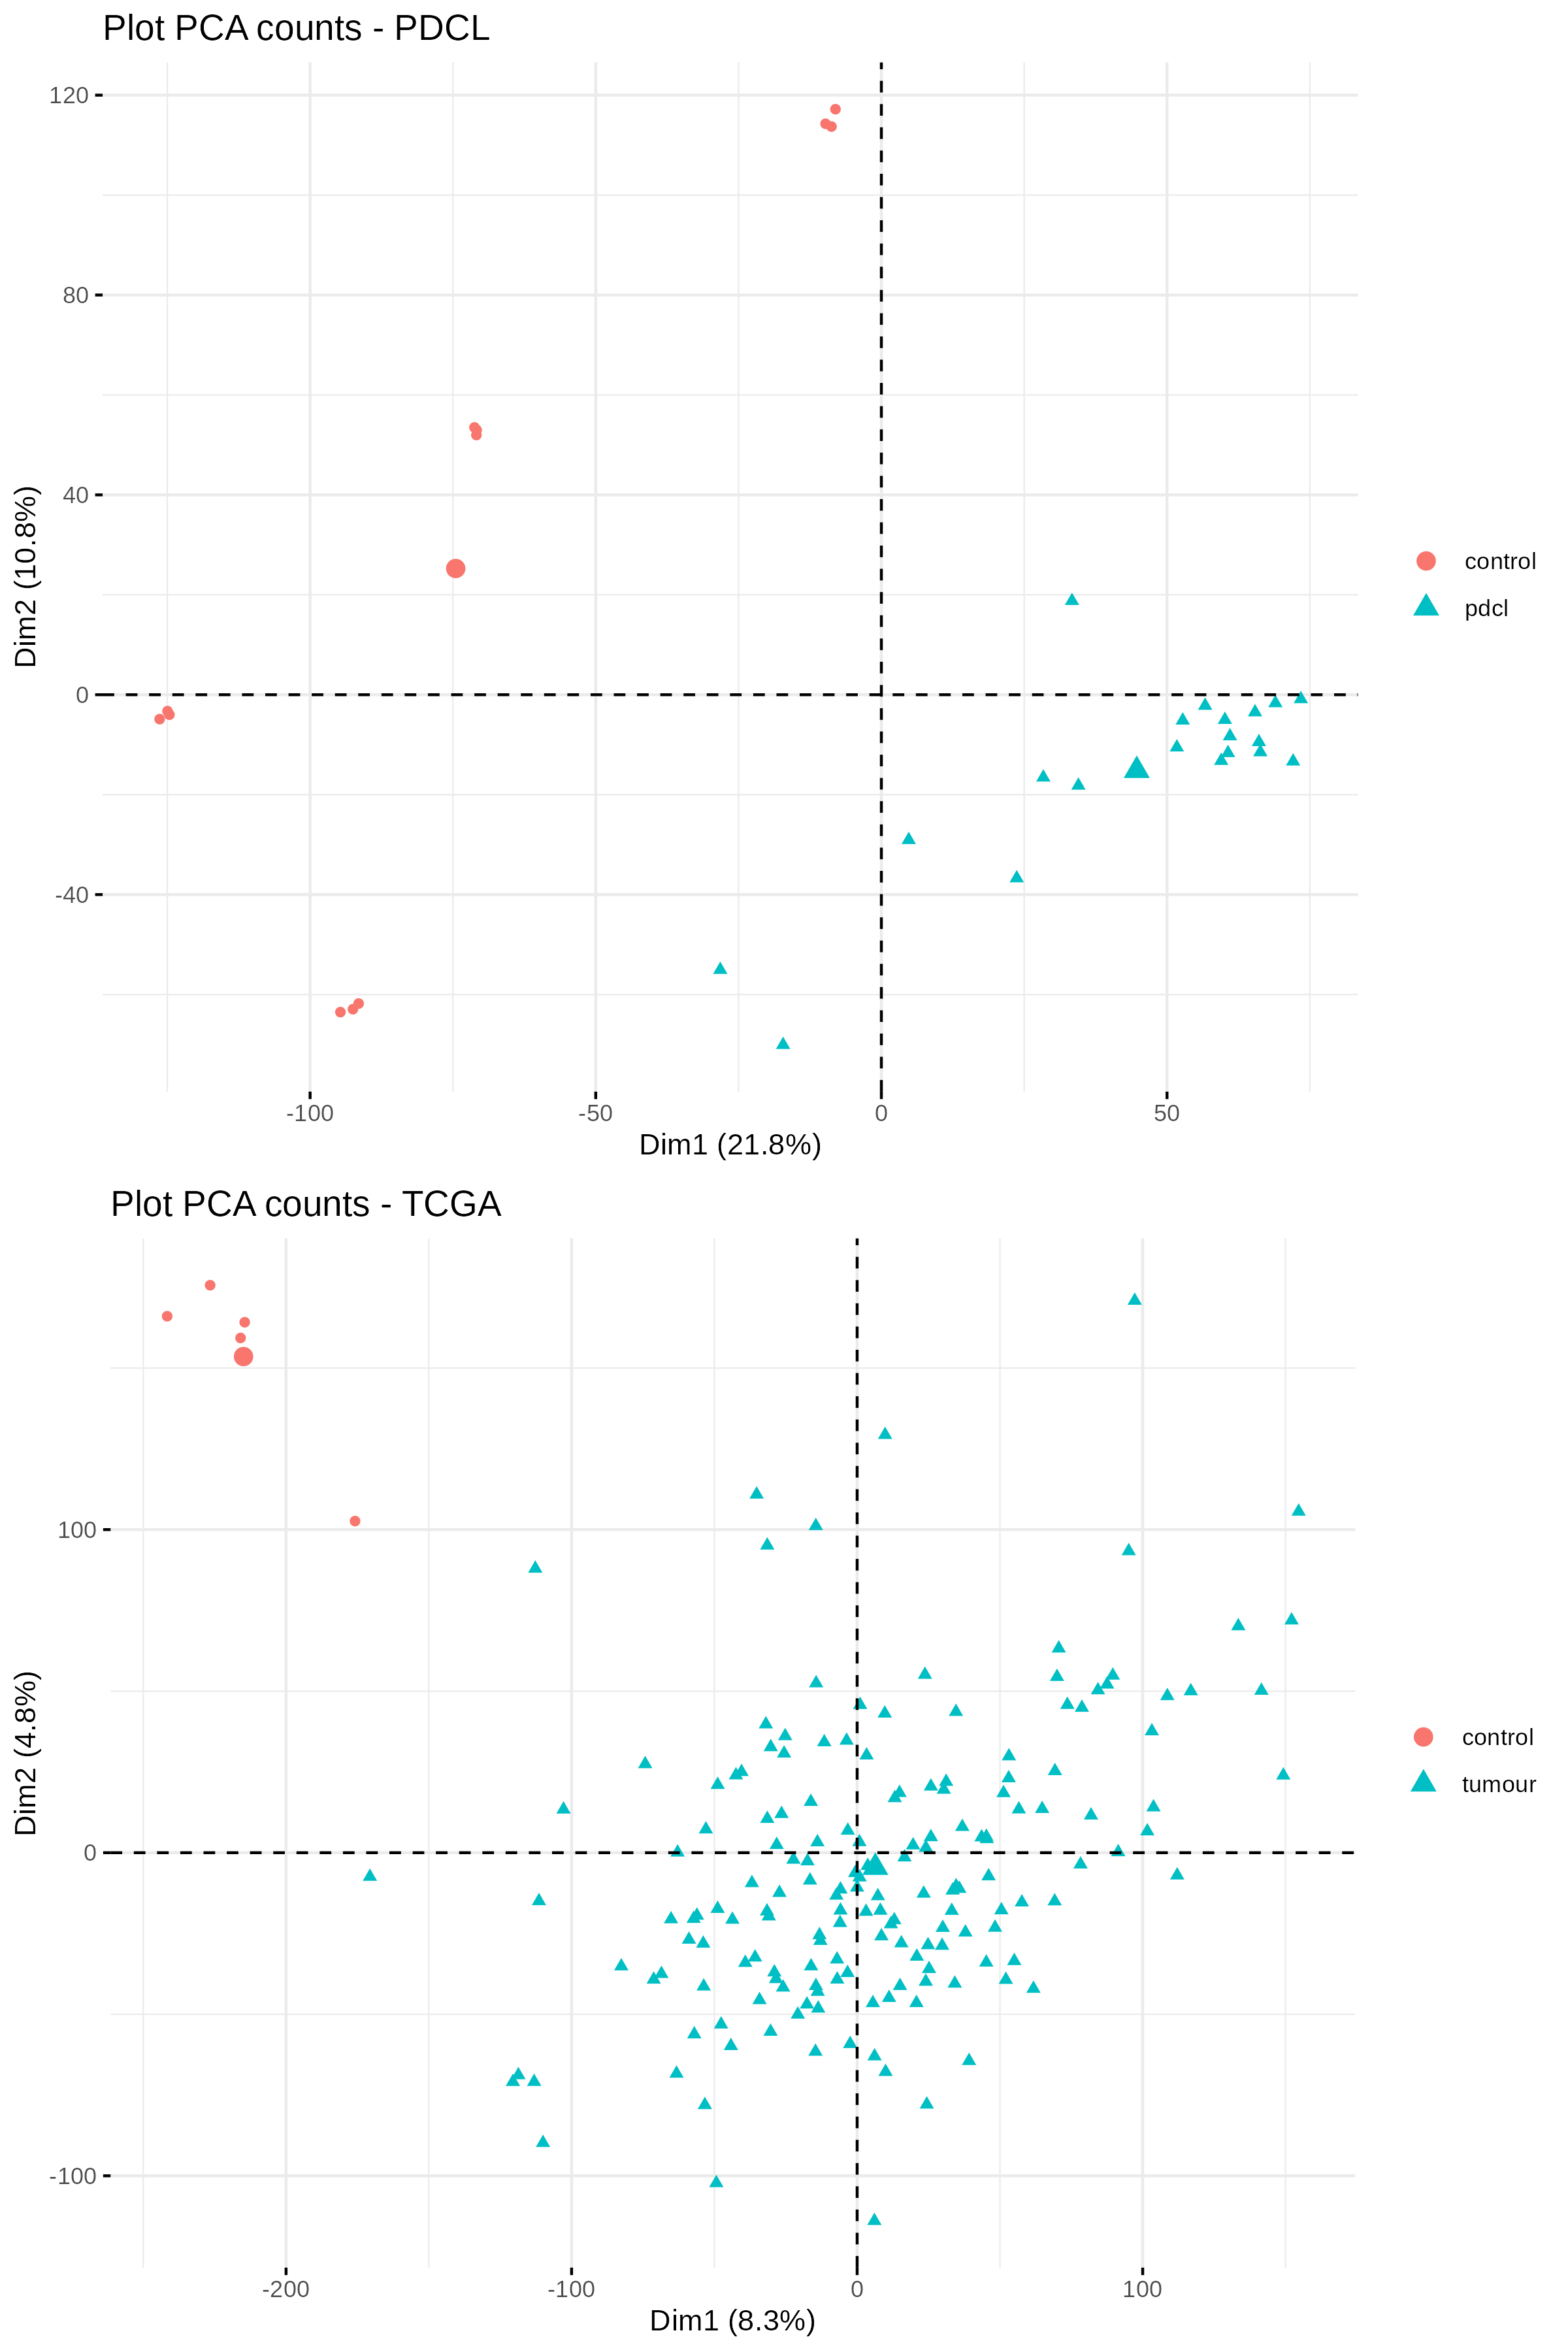
\includegraphics[height=0.8\textheight]{img/pca_plot}
        \caption{
            Plot of the \acrshort{pca} on the normalized counts of control and glioblastoma samples of the \acrshort{pdcl} and \acrshort{tcga} datasets.
        }
        \label{fig:pca-plot}
    \end{center}
\end{figure}

Figure \ref*{fig:pca-plot} shows the results of a \acrfull{pca} performed on the normalized count value.
It can be seen that the controls are separated from the tumours in both the \acrshort{pdcl} and the \acrshort{tcga} datasets by the first two components of the \acrshort{pca}.
The first component explains more variances in the data in the \acrshort{pdcl} datasets with 21\% compared to 8\% with \acrshort{tcga}.
In the \acrshort{tcga} datasets, the tumour samples tend to spread more across the second component than the controls which seem to pack together while in the \acrshort{pdcl} dataset, controls are more scattered. 

\begin{figure}
    \begin{center}
        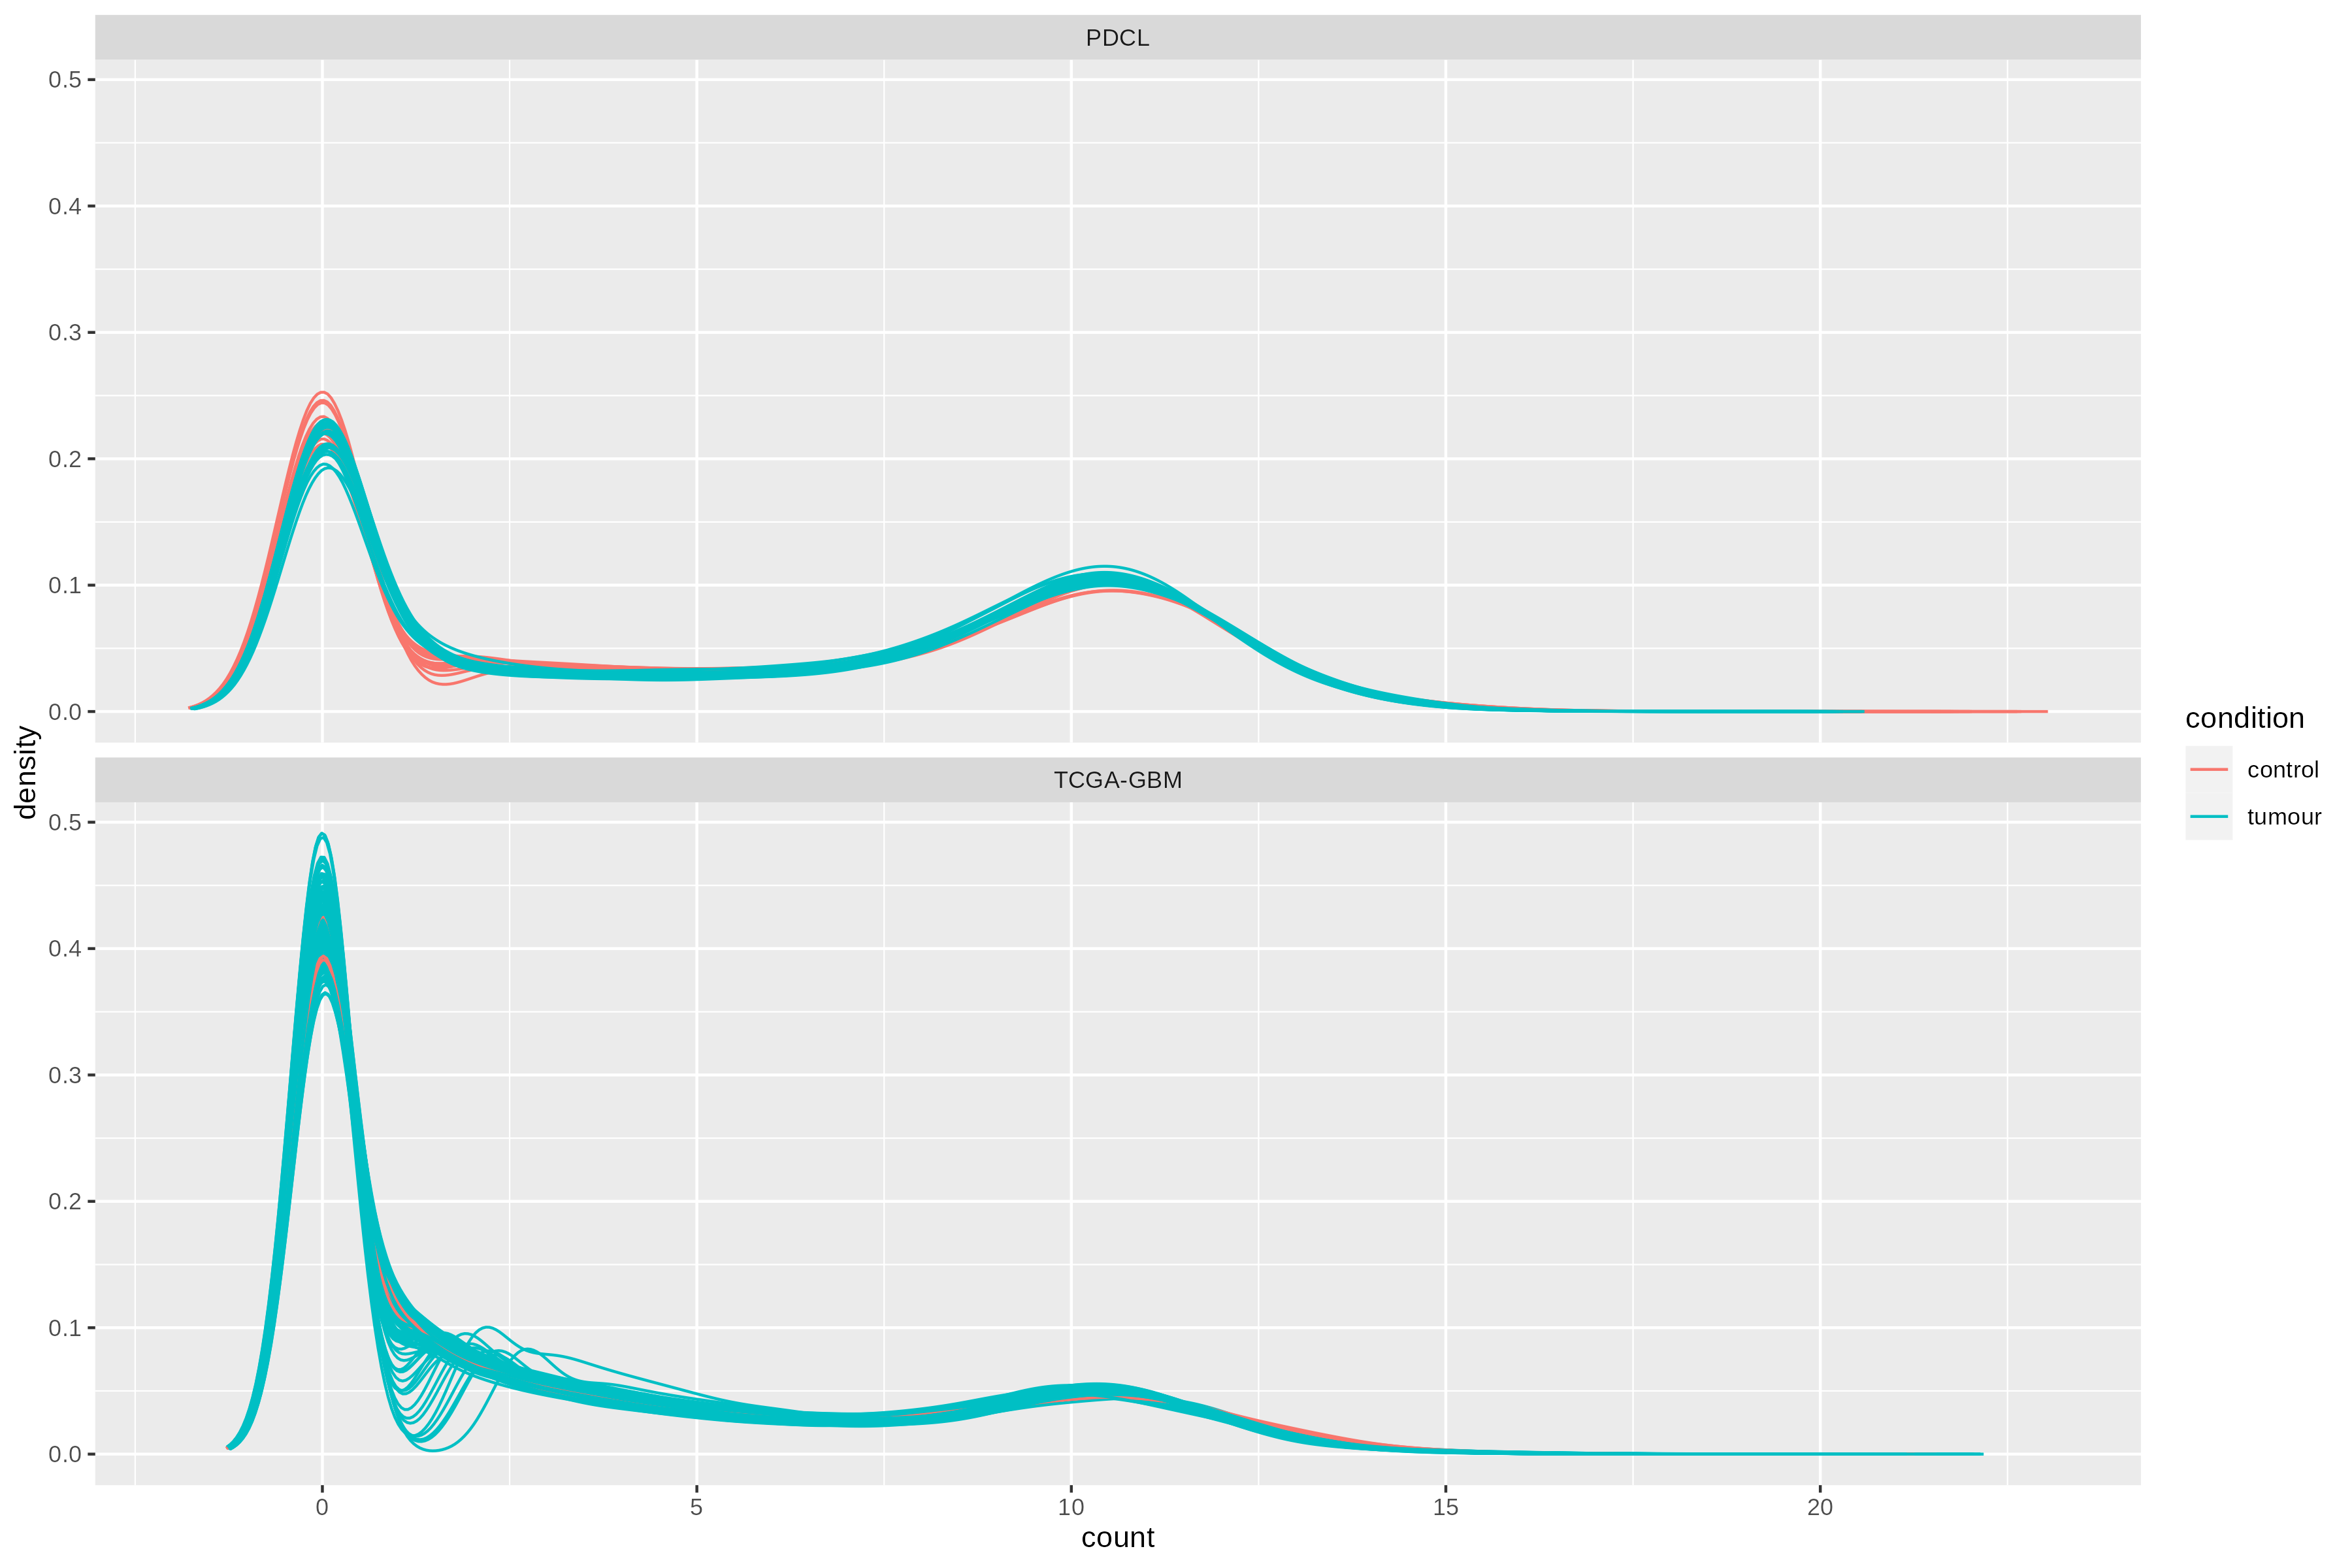
\includegraphics[width=0.8\textwidth]{img/density_plot}
        \caption{
            Plot of the density of the normalized counts in control and glioblastoma samples of the \acrshort{pdcl} and \acrshort{tcga} datasets.
            Each curve represents a different sample.
        }
        \label{fig:density-plot}
    \end{center}
\end{figure}

Figure \ref*{fig:density-plot} shows the distribution of normalized gene counts in controls and tumours among both datasets.
The distribution of counts is similar among controls and tumours in both datasets with a similar intensity on the peak between controls and tumours with respect to the dataset.
The first peak corresponds to genes with a low expression and the second one to genes with a high expression.
For information, \acrshort{penda} uses a bimodal distribution to find the value of the first peak and filter out genes with a low expression.
Together, these data seem to indicate that the controls chosen are suitable to perform the \acrlong{de} analysis and then pathway enrichment.

\subsection{Analysis of the deregulated pathways at the patient population scale}

\subsubsection{Target pathways show decreased significance introduced biological variability}

The \acrshort{kegg} database includes many disease-related pathways, including glioma.
Such pathways can be used as targets to validate enrichment results in datasets derived from the same condition.
For example, Zyla \textit{et al} used the adjusted p-value of the \textit{Glioma} entry (path:hsa05214) as a target pathway to assess the sensitivity of different ranking metrics when studying microarray data from brain tissue \cite*{Zyla2017}.
Here, as we are comparing RNA-Seq data from glioblastoma samples to normal controls, we should expect the adjusted p-value (\acrshort{fdr} in this study) to be below our defined threshold.
The \acrshort{fdr} value for \textit{Glioma} is 0.053 in G:Profiler and 0.83 in \acrshort{gsea} for the \acrshort{pdcl} dataset.
With \acrshort{tcga} data, the \acrshort{fdr} value for \textit{Glioma} is 0.0009 in G:Profiler and 0.005 in \acrshort{gsea}.
Controls for the \acrshort{pdcl} dataset are taken from another study \cite*{Lundin2018}, introducing experimental and biological variability independent from disease deregulation.
Furthermore, some replicates in the controls of the \acrshort{pdcl} datasets come from astrocytoma cell lines.
It shows that a good set of controls can influence the quality of the results given.

\subsubsection{Differences in deregulated categories across pathway databases and enrichment algorithms}

\begin{figure}
    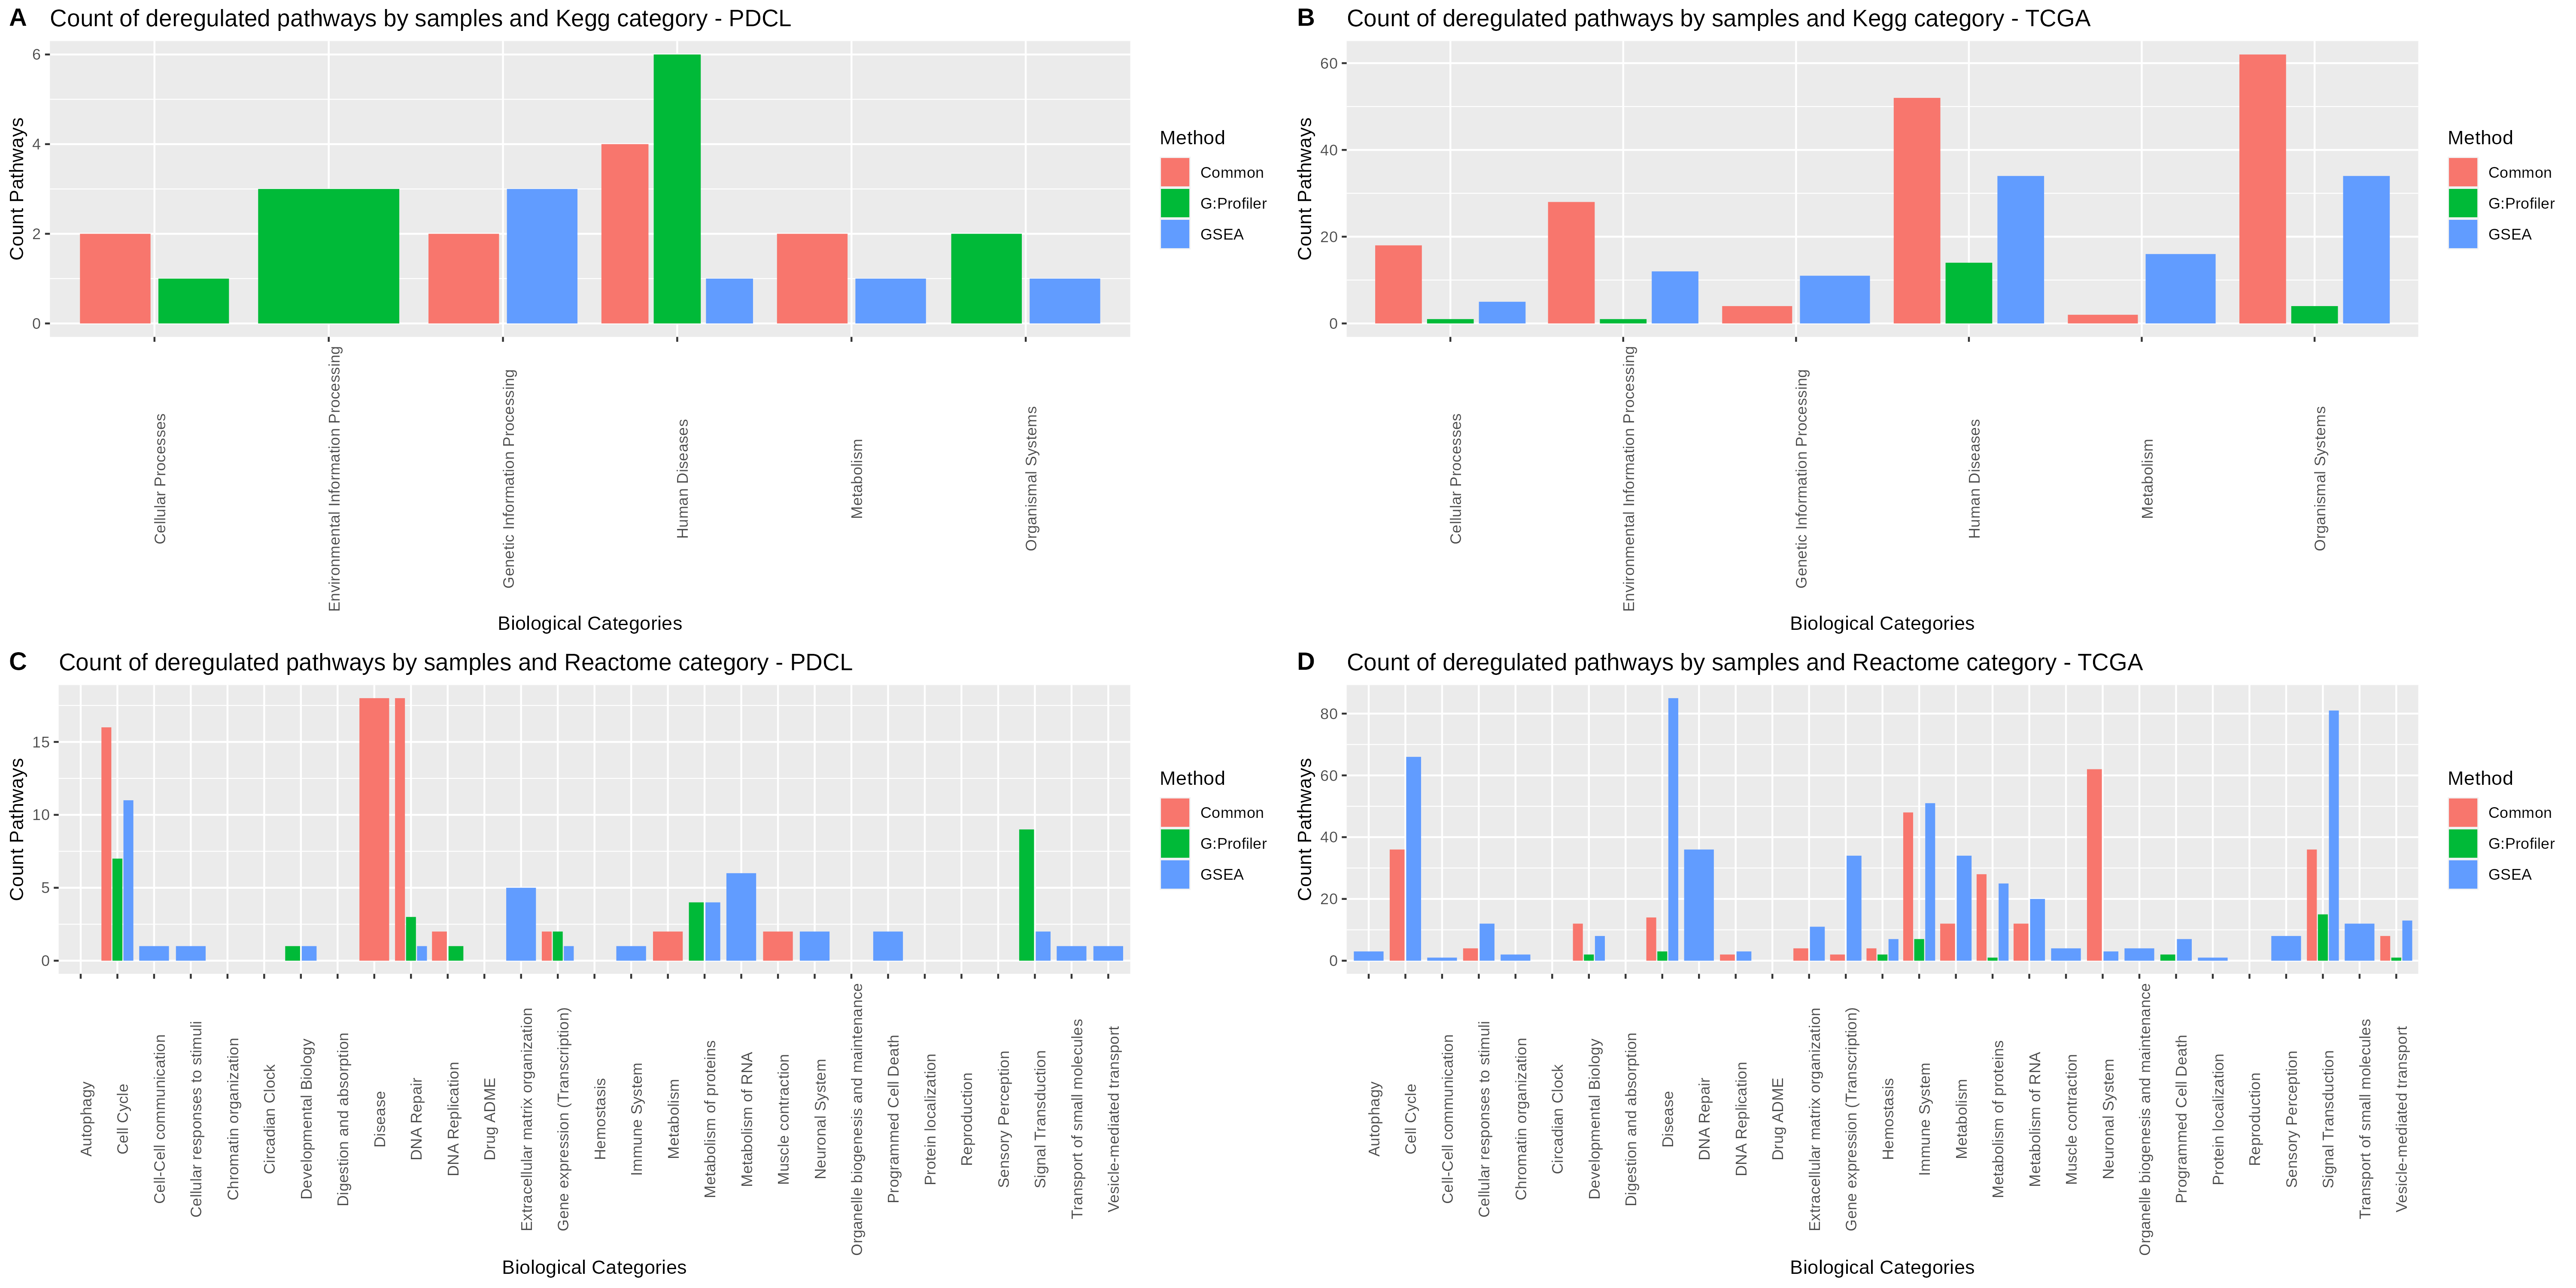
\includegraphics[width=\textwidth]{img/barplot-categ-global}
    \caption{
        Barplot of the count of significantly deregulated pathways for (A) \acrshort{kegg} categories in \acrshort{pdcl}; (B) \acrshort{kegg} categories in \acrshort{tcga}; (C) Reactome categories in \acrshort{pdcl}; (D) Reactome categories in \acrshort{tcga}.
        Pathways are coloured whether they are specific to G:Profiler or \acrshort{gsea}, they are significantly enriched in one of the tools, or common, they are significantly enriched in both tools.
    }
    \label{fig:barplot-categ-global}
\end{figure}

As can be seen in figure \ref*{fig:barplot-categ-global}, G:Profiler and \acrshort{gsea} yield different results which are also influenced by the database chosen.
We recommend investigating more than one database when performing pathway enrichment as the choice of the database may impact the results \cite*{Mubeen2019}.
Most of the time, more pathways are significantly enriched in \acrshort{gsea} compared to G:Profiler.
In some cases, there is no correlation between G:Profiler and \acrshort{gsea} results.
For example, the \textit{Organismal Systems} \acrshort{kegg} category is only enriched with pathways specific to G:Profiler or to \acrshort{gsea} with \acrshort{pdcl} data.
Still with the same dataset and database, the \textit{Environmental information Processing} category is only found enriched with G:profiler.
Inversely, the \textit{Disease} Reactome category is enriched with only pathways found by both G:Profiler and \acrshort{gsea} in \acrshort{pdcl} data.
In addition, Reactome categories like \textit{Circadian Clock} or \textit{Reproduction} are not found enriched in any of the datasets nor tools.
In this study, pathways in the \acrshort{gmt} are filtered only on their size.
Yet, it may be beneficial to remove pathways which are not involved in the biological condition being investigated.
The \acrshort{fdr} multiple hypothesis correction method is influenced by the number of null-hypotheses tested, here the number of genes tested for differential expression or pathway tested for enrichment.
Therefore, the more pathways are being tested, the stronger the correction applied to the p-value is.

\subsubsection{Investigation of selected pathways}

\acrshort{fdr} values for different pathways from \acrshort{kegg} and Reactome given by G:Profiler and \acrshort{gsea} in both datasets is presented in figure \ref*{supp:heatmap-fdr-global}.
\begin{figure}
    \begin{center}
        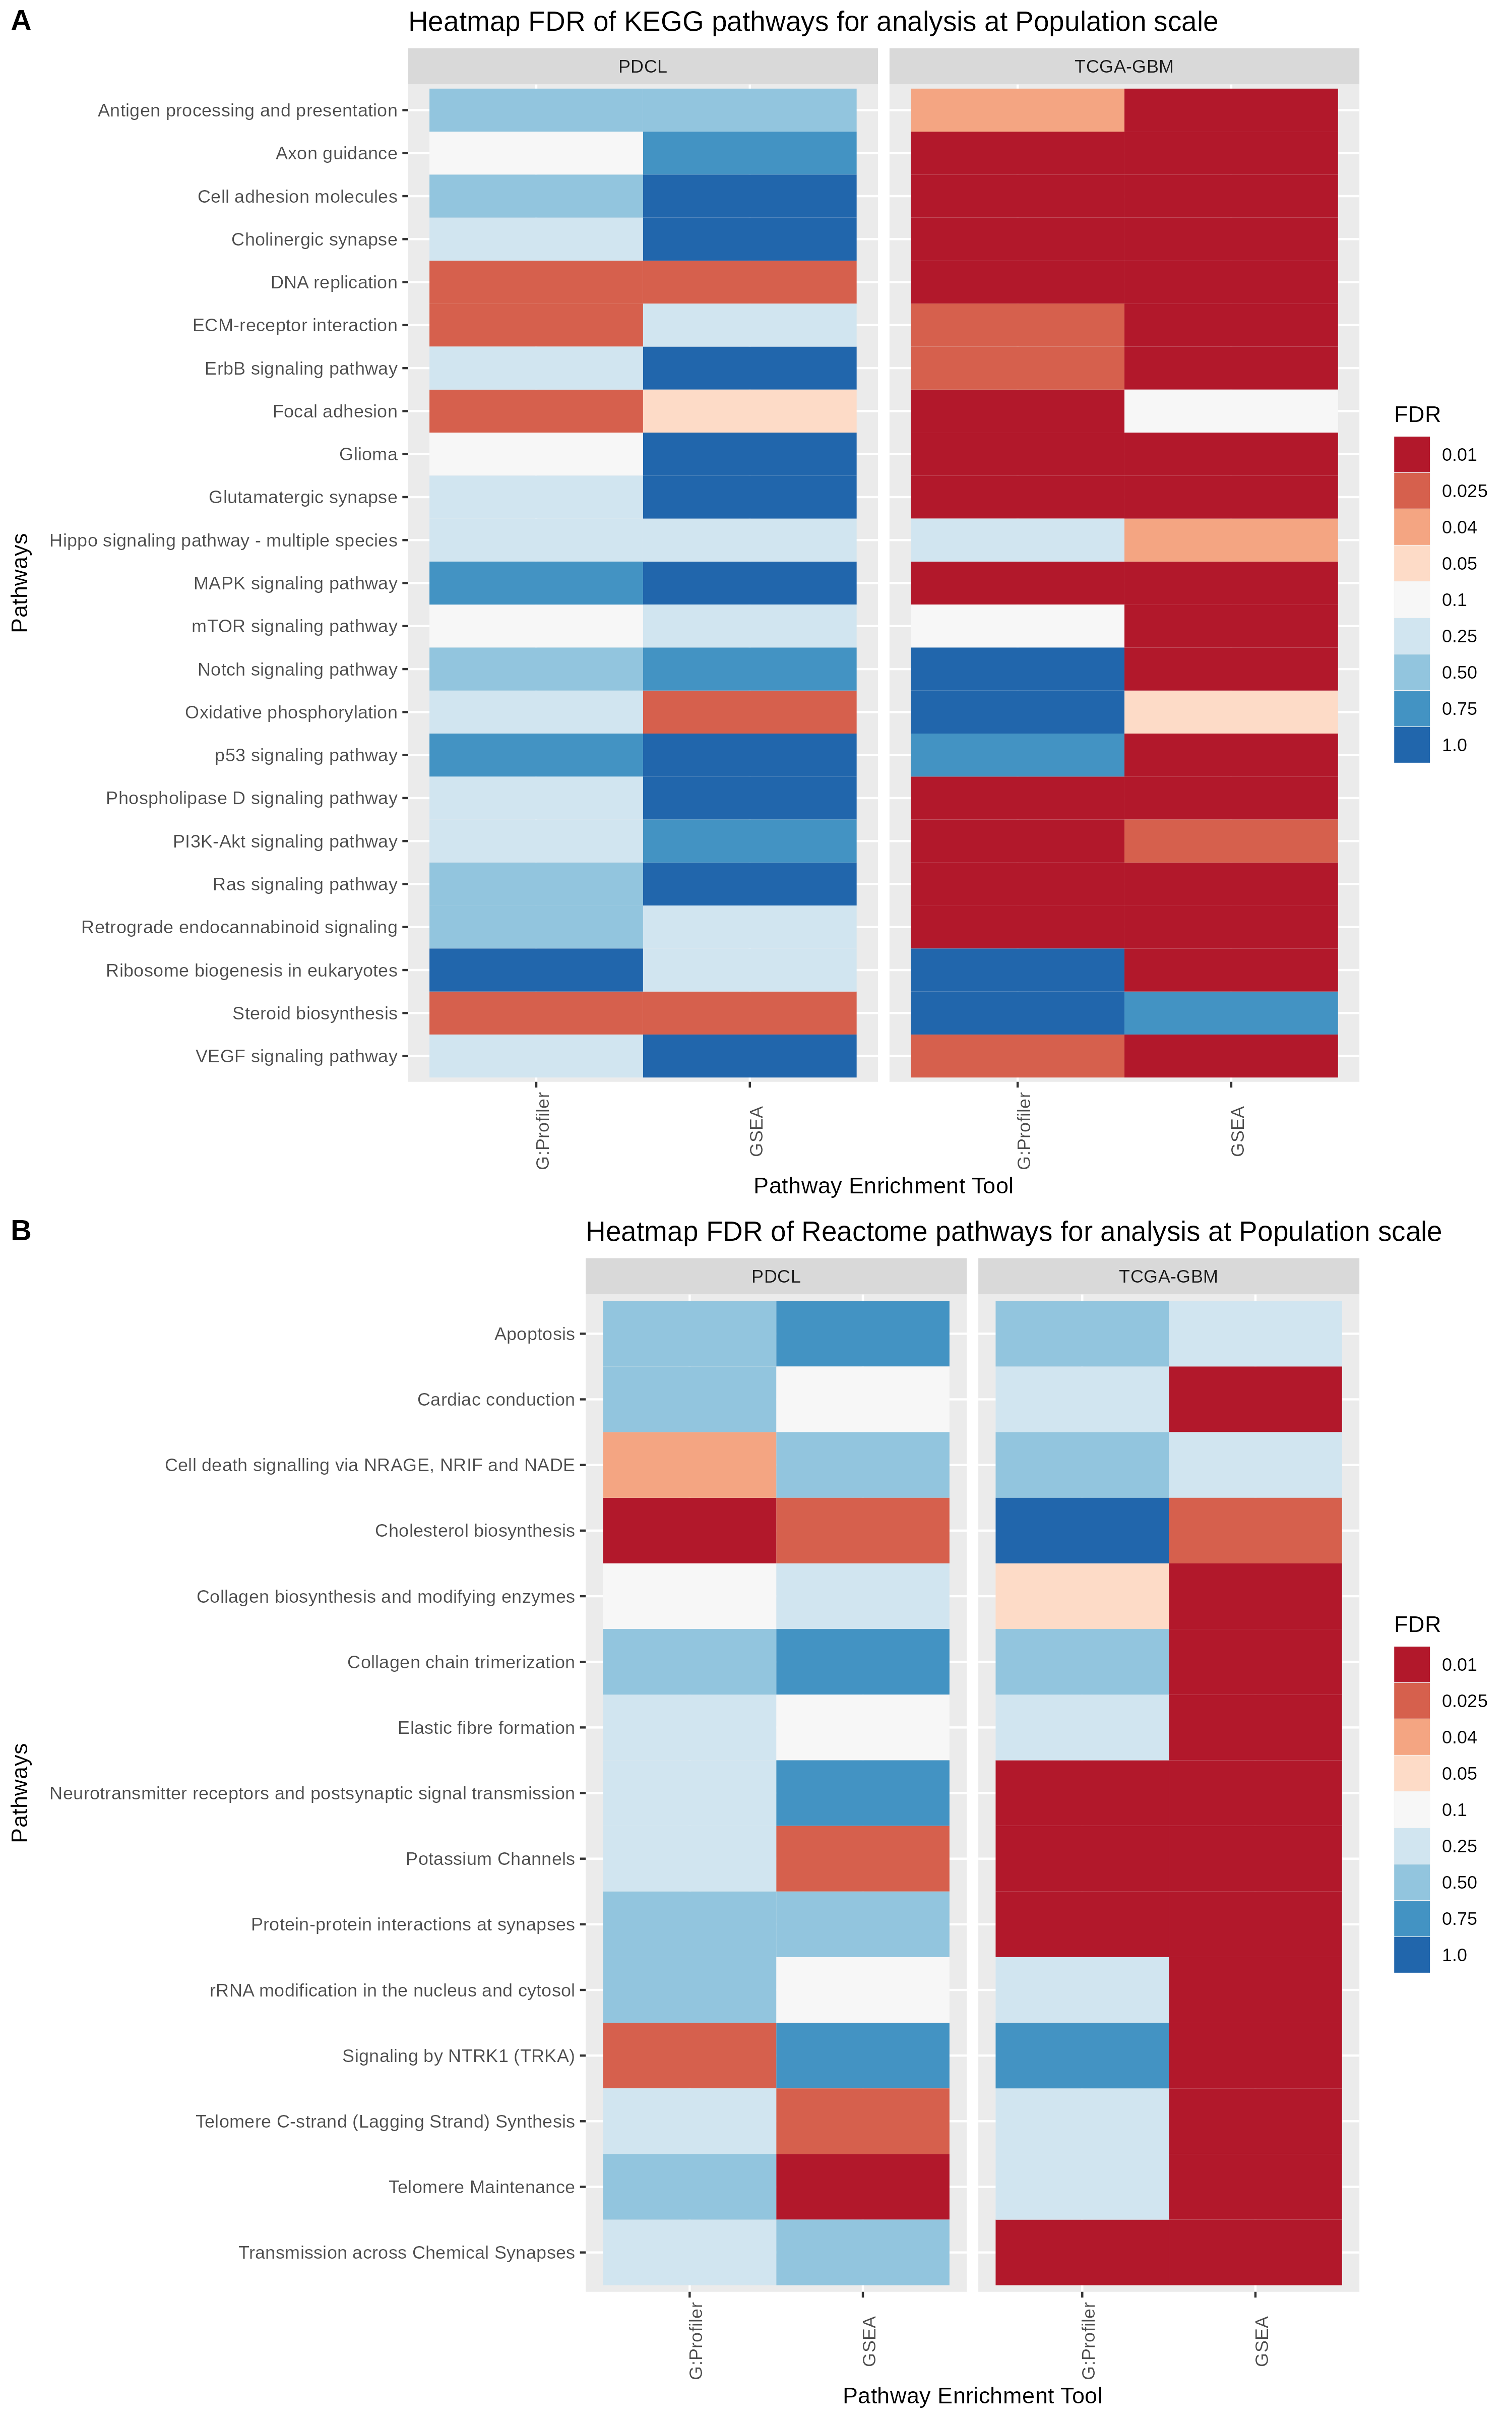
\includegraphics[height=0.7\paperheight]{img/heatmap-fdr-global}
        \caption{
            Heatmap of deregulated pathways in the \acrshort{pdcl} and the \acrshort{tcga} datasets for (A) the \acrshort{kegg} database and (B) the Reactome database.
            \acrshort{fdr} values below 5\% are considered significant (red) and they are not considered significant if greater than 5\% (blue).
        }
        \label{supp:heatmap-fdr-global}
    \end{center}
\end{figure}
As before, we see that a same pathways can be found enriched in one enrichment tool but not in another.
For example, the \acrshort{fdr} for \textit{Oxidative phosphorylation} is significant in both datasets with \acrshort{gsea} but not with G:Profiler.
In \acrshort{tcga}, the \textit{p53 signalling} pathway is found significant only with \acrshort{gsea} and it is not enriched with \acrshort{pdcl} data.
Yet it is found deregulated in one sample during the personalized analysis of \acrshort{pdcl} samples (described below) suggesting it is rather due to the dataset.
Using pathway enrichment we can also highlight the differences between both datasets.
As an example, many well-known signalling pathways such as \textit{PI3K-Akt signalling}, \textit{RAS signalling} and \textit{VEGF signalling} are found enriched only in \acrshort{tcga}.
On the opposite, pathways involved in cholesterol metabolism such as \textit{Steroid biosynthesis} and \textit{Cholesterol biosynthesis} are found enriched only in \acrshort{pdcl}.
We will show below, that we can assess which samples are associated with an altered cholesterol synthesis.

\subsection{Analysis of the deregulated pathways at the individual level}

\subsubsection{Cell adhesion to the ECM is the most frequently deregulated pathway in PDCL samples}

Table \ref*{table:frequently-dereg-pathways-kegg} and \ref*{table:frequently-dereg-pathways-reactome} show the most frequently deregulated pathways in \acrshort{pdcl}.
The \textit{Focal adhesion} (path:hsa04510) is the most frequently deregulated \acrshort{kegg} pathway with 13 samples affected while \textit{Transmission across Chemical Synapses} (R-HSA-112315) is the most frequently deregulated Reactome pathway with 5 samples affected.
Results contain pathways linked to processes influencing the cell motility and its fixation on the matrix such as: \textit{Focal adhesion} (path:hsa04510), \textit{ECM-receptor interaction} (path:hsa04512), \textit{Cell adhesion molecules} (path:hsa04514), \textit{Collagen synthesis} (R-HSA-165814, R-HSA-8948216) and \textit{elastic fibre formation} (R-HSA-1566948).
Glioblastoma cells have the ability to migrate and invade surrounding tissue, sometimes migrating to other organs as well \cite*{Lah2020}, supporting the validity of these results.

In a similar way, \textit{Steroid biosynthesis} and \textit{Cholesterol biosynthesis} are found deregulated in 4 and 3 different samples, respectively.
\textit{Cholesterol metabolism} has been documented in the literature to be affected in the case of glioblastoma.

The \textit{Oxidative phosphorylation} (path:hsa00190), well-known for its role in the generation of \acrshort{atp}, is found deregulated in 4 samples.
This pathway has been widely studied due to its important role in the generation of \acrshort{atp} and its potential implication in the Warburg Effect, an increased use of glycolysis to produce \acrshort{atp} even though oxygen is available \cite*{Spinicci2022}.
It was first hypothesized that mitochondria were defective in tumour cells, yet it was later shown that mitochondrial function in cancer cells was similar to normal cells \cite*{Cairns2011}.
The \textit{Hippo signalling pathway} (path:hsa04392, path:hsa04390) and \textit{Retrograde endocannabinoid signalling} (path:hsa04723), two signalling pathways whose role in cancer have been documented in the literature, are found deregulated in 6 and 5 different samples, respectively \cite*{Wei2014,Liu2018,BasuRoy2015}.

\begin{table}
    \centering
    \resizebox*{\textwidth}{!}{
        \begin{tabular}{ |c|c|c|c|c| }
            \hline
            Database & Pathway ID & Description & Category & Number of PDCL \\
            \hline
            KEGG & path:hsa04510 & Focal adhesion & Cellular Processes & 13 \\
            KEGG & path:hsa04360 & Axon guidance & Organismal Systems & 10 \\
            KEGG & path:hsa04512 & ECM-receptor interaction & Environmental Information Processing & 5 \\
            KEGG & path:hsa04724 & Glutamatergic synapse & Organismal Systems & 5 \\
            KEGG & path:hsa04725 & Cholinergic synapse & Organismal Systems & 5 \\
            KEGG & path:hsa00100 & Steroid biosynthesis & Metabolism & 4 \\
            KEGG & path:hsa00190 & Oxidative phosphorylation & Metabolism & 4 \\
            KEGG & path:hsa04612 & Antigen processing and presentation & Organismal Systems & 4 \\
            KEGG & path:hsa04723 & Retrograde endocannabinoid signalling & Organismal Systems & 4 \\
            KEGG & path:hsa03008 & Ribosome biogenesis in eukaryotes & Genetic Information Processing & 3 \\
            KEGG & path:hsa04012 & ErbB signalling pathway & Environmental Information Processing & 3 \\
            KEGG & path:hsa04072 & Phospholipase D signalling pathway & Environmental Information Processing & 3 \\
            KEGG & path:hsa04392 & Hippo signalling pathway - multiple species & Environmental Information Processing & 3 \\
            KEGG & path:hsa04514 & Cell adhesion molecules & Environmental Information Processing & 3 \\
            KEGG & path:hsa04714 & Thermogenesis & Organismal Systems & 3 \\
            \hline
        \end{tabular}
    }
    \caption{
        Table of the frequently \acrshort{kegg} pathways deregulated in the \acrshort{pdcl}.
        \textit{Focal adhesion} is the most frequently deregulated pathway with 13 samples affected.
    }
    \label{table:frequently-dereg-pathways-kegg}
\end{table}

\begin{table}
    \centering
    \resizebox*{\textwidth}{!}{
        \begin{tabular}{|c|c|c|c|c|}
            \hline
            Database & Pathway ID & Description & Category & Number of PDCL \\
            \hline
            Reactome & R-HSA-112315 & Transmission across Chemical Synapses & Neuronal System & 5 \\
            Reactome & R-HSA-1650814 & Collagen biosynthesis and modifying enzymes & Extracellular matrix organization & 4 \\
            Reactome & R-HSA-5576891 & Cardiac conduction & Muscle contraction & 4 \\
            Reactome & R-HSA-8948216 & Collagen chain trimerization & Extracellular matrix organization & 4 \\
            Reactome & R-HSA-112314 & Neurotransmitter receptors and postsynaptic signal transmission & Neuronal System & 3 \\
            Reactome & R-HSA-191273 & Cholesterol biosynthesis & Metabolism & 3 \\
            Reactome & R-HSA-6790901 & rRNA modification in the nucleus and cytosol & Metabolism of RNA & 3 \\
            Reactome & R-HSA-6794362 & Protein-protein interactions at synapses & Neuronal System & 3 \\
            Reactome & R-HSA-109581 & Apoptosis & Programmed Cell Death & 2 \\
            Reactome & R-HSA-1296071 & Potassium Channels & Neuronal System & 2 \\
            Reactome & R-HSA-1566948 & Elastic fibre formation & Extracellular matrix organization & 2 \\
            Reactome & R-HSA-157579 & Telomere Maintenance & Cell Cycle & 2 \\
            Reactome & R-HSA-174417 & Telomere C-strand (Lagging Strand) Synthesis & Cell Cycle & 2 \\
            Reactome & R-HSA-187037 & Signalling by NTRK1 (TRKA) & Signal Transduction & 2 \\
            Reactome & R-HSA-204998 & Cell death signalling via NRAGE, NRIF and NADE & Signal Transduction & 2 \\
            \hline
        \end{tabular}
    }
    \caption{
        Table of the frequently Reactome pathways deregulated in the \acrshort{pdcl}.
        \textit{Transmission across Chemical Synapses} is the most frequently deregulated pathway with 5 samples affected.
        Collagen pathways are deregulated in 4 different samples.
    }
    \label{table:frequently-dereg-pathways-reactome}
\end{table}

\begin{figure}
    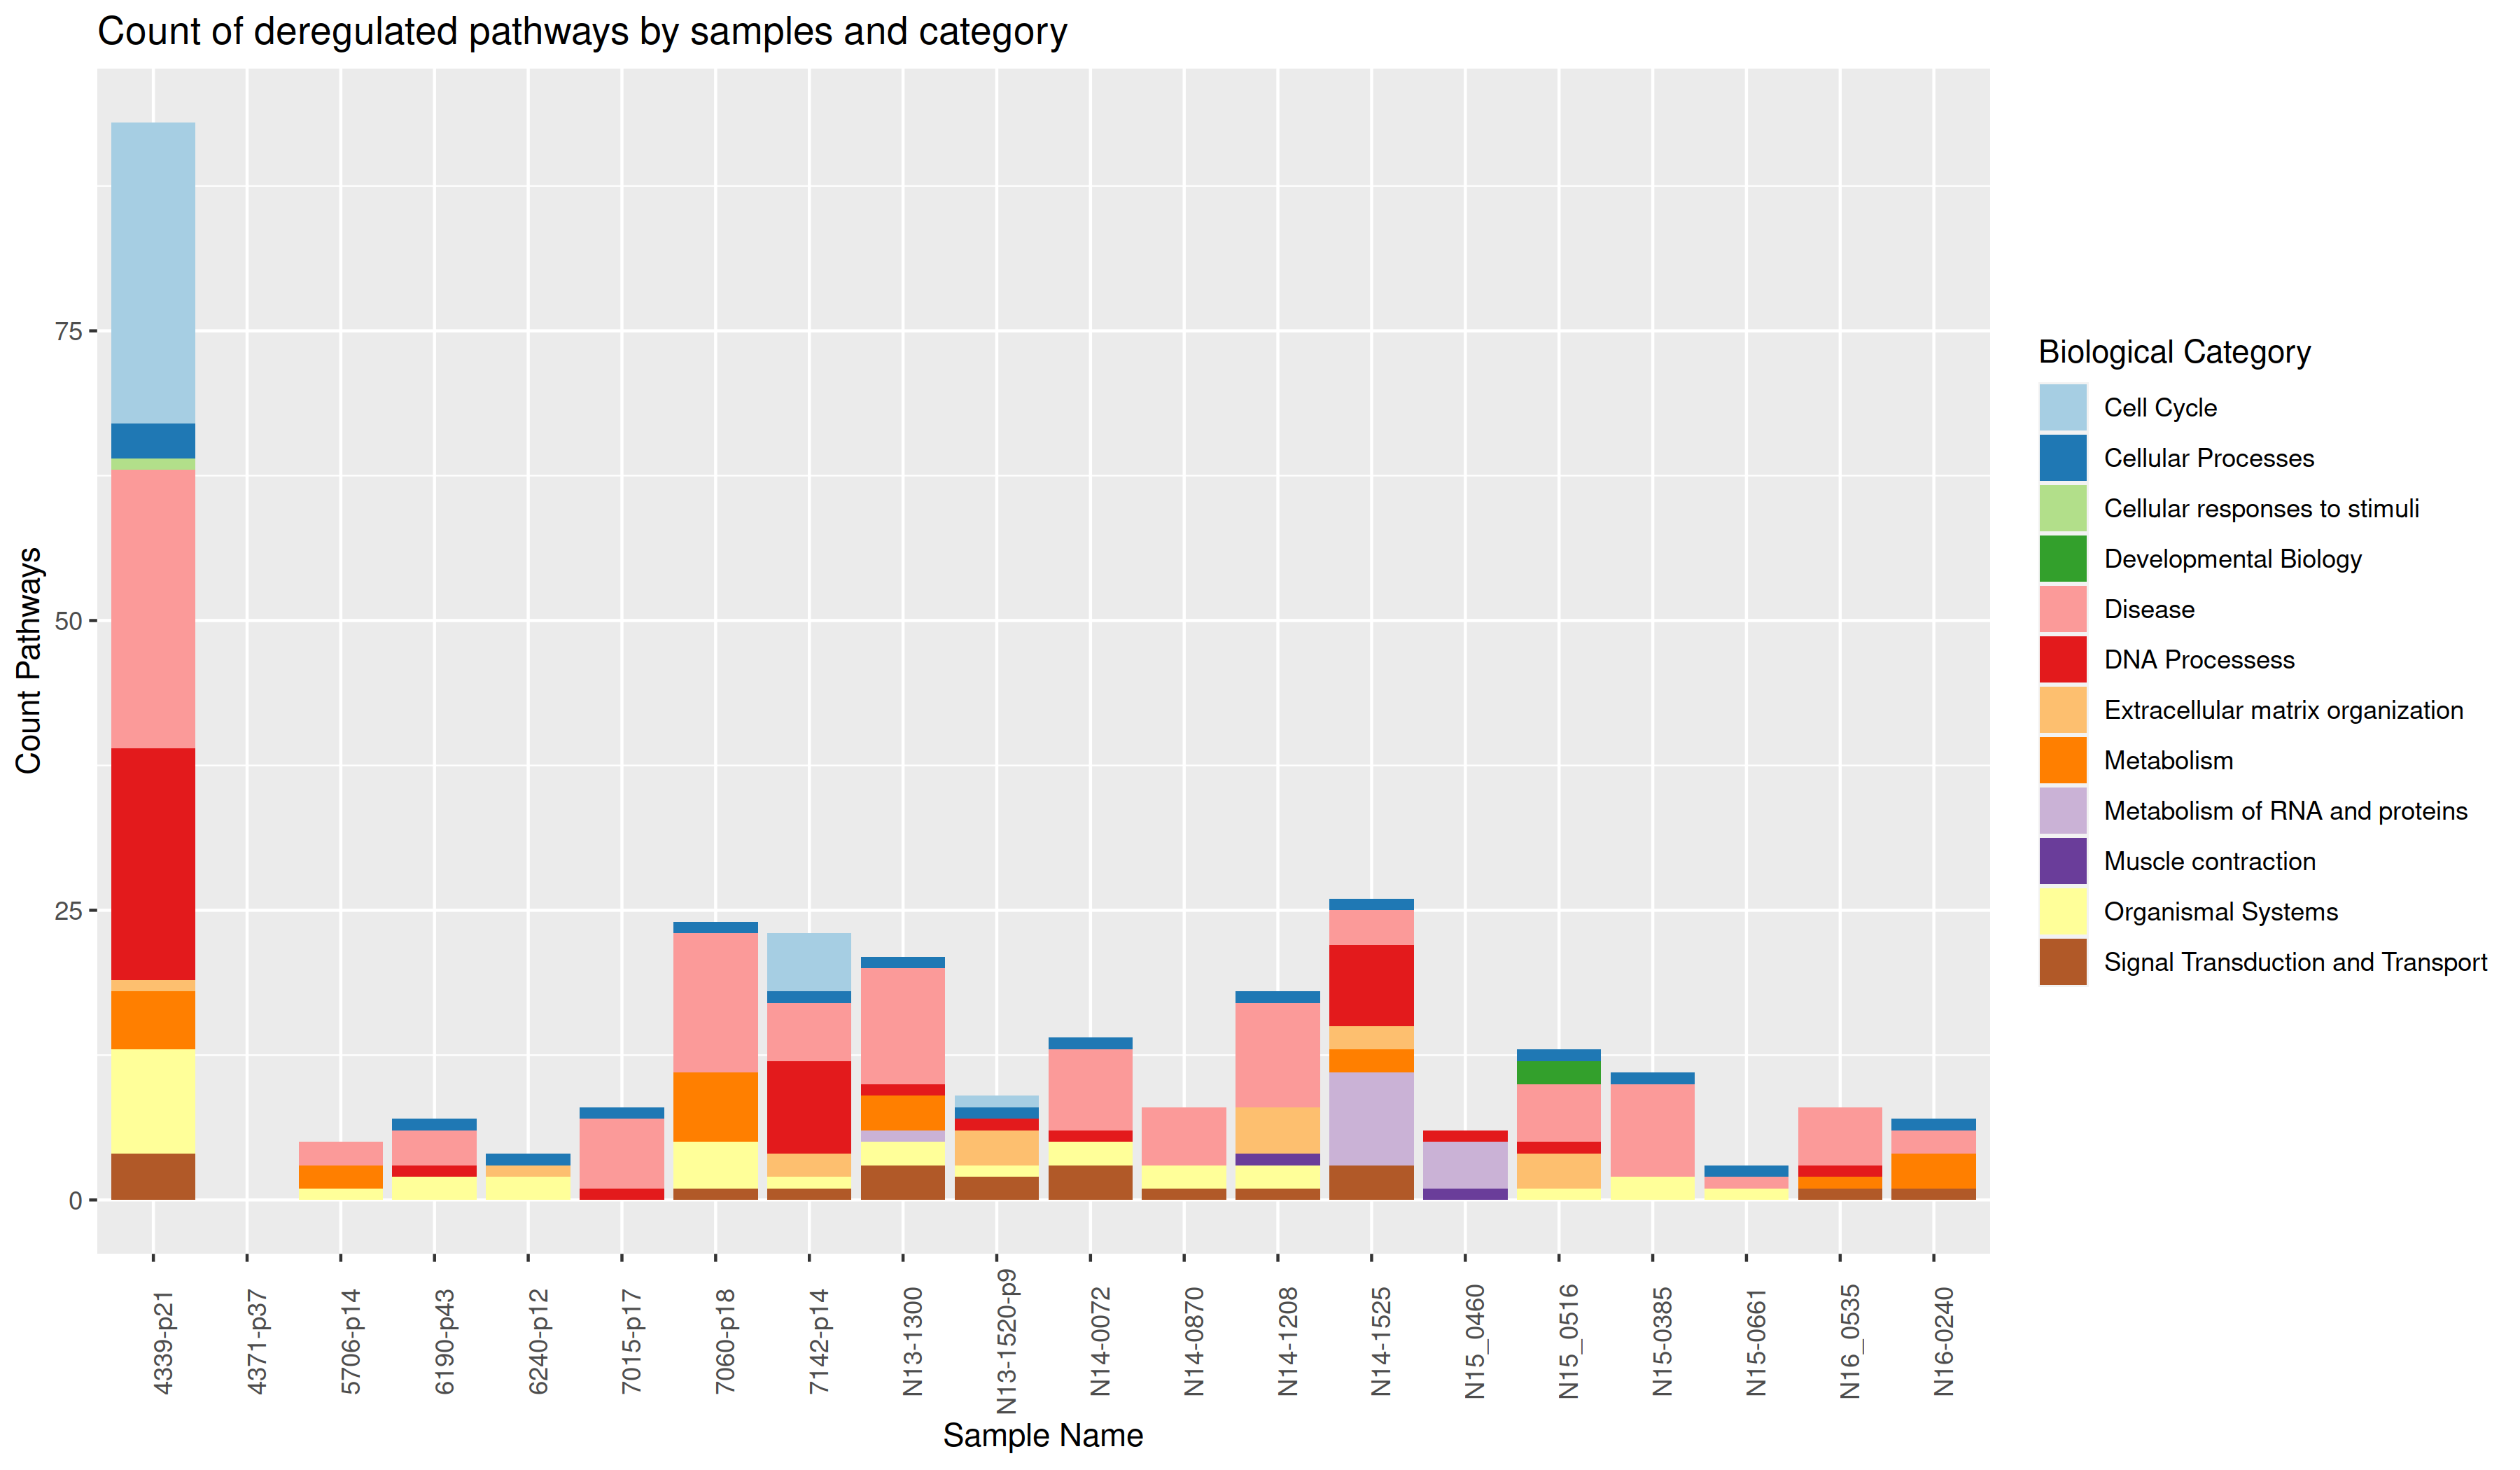
\includegraphics[width=\textwidth]{img/barplot-categ-pdcl}
    \caption{
        Number of deregulated pathways per category and per sample in the \acrshort{pdcl} dataset.
        The  \textit{Human Diseases} and \textit{Organismal Systems} categories are the most frequently deregulated \acrshort{kegg} categories.
        In Reactome, deregulated pathways are often associated with \textit{Neuronal System}, \textit{DNA Repair/Replication} and \textit{Signal Transduction}.
        \textit{4339-p21} is the sample with the most deregulated pathways in both \acrshort{kegg} and reactome.
        Pathways in this sample are associated with the \textit{Cellular Processes} and \textit{Environmental/Genetic Information Processing} \acrshort{kegg}, or the \textit{Cell-Cycle} Reactome category.
    }
    \label{fig:barplot-categ-pdcl}
\end{figure}

As can be seen in figure \ref*{fig:barplot-categ-pdcl}, the sample \textit{4339-p21} is the most deregulated with around 40 pathways significantly enriched in both \acrshort{kegg} and Reactome.
Most of the pathways found deregulated with the \acrshort{kegg} database, across all the \acrshort{pdcl} samples, are associated with \textit{Human Diseases}.
\textit{Human Diseases} aside, the majority of deregulated pathways in the sample \textit{4339-p21} are associated to the \textit{Cellular Processes} and \textit{Environmental/Genetic Information Processing} \acrshort{kegg}, or the \textit{Cell-Cycle} Reactome category.

\subsubsection{Pathways linked to the Cell-Cycle and the ECM interactions are the most frequently deregulated in TCGA-GBM samples}

Tables \ref*{table:frequently-dereg-pathways-kegg-tcga} and \ref*{table:frequently-dereg-pathways-reactome-tcga} show the most frequently deregulated pathways in the \acrshort{tcga} dataset.
While \textit{Focal adhesion} was the most frequently altered \acrshort{kegg} pathway among the \acrshort{pdcl} samples, it is fourth with \acrshort{tcga}.
Furthermore, no pathways linked to the metabolism appear in the table for \acrshort{kegg} pathways.
As expected, the \textit{p53 signalling} pathway is frequently altered with 118 samples out of 169 samples affected.
Similar to the result obtained with \acrshort{pdcl} samples, 3 Reactome pathways linked to the collagen protein synthesis are among the pathways often deregulated.
Still with the Reactome database, 3 pathways involved in the \textit{Cell-Cycle} are deregulated in at least 149 samples and seem to indicate that the \textit{G1/S Phase Transition} is the main part of the cell cycle affected by glioblastoma.

\begin{table}
    \centering
    \resizebox*{\textwidth}{!}{
        \begin{tabular}{ |c|c|c|c|c| }
            \hline
            Database & Pathway ID & Description & Category & Number of Samples \\
            \hline
            KEGG & path:hsa04110 & Cell Cycle & Cellular Processes & 153 \\
            KEGG & path:hsa04512 & ECM-receptor interaction & Environmental Information Processing & 147 \\
            KEGG & path:hsa04145 & Phagosome & Cellular Processes & 130 \\
            KEGG & path:hsa04510 & Focal adhesion & Cellular Processes & 129 \\
            KEGG & path:hsa03030 & DNA replication & Genetic Information Processing & 126 \\
            KEGG & path:hsa04640 & Hematopoietic cell lineage & Organismal Systems & 125 \\
            KEGG & path:hsa04672 & Intestinal immune network for IgA production & Organismal Systems & 125 \\
            KEGG & path:hsa04514 & Cell adhesion molecules & Environmental Information Processing & 124 \\
            KEGG & path:hsa04612 & Antigen processing and presentation & Organismal Systems & 124 \\
            KEGG & path:hsa03010 & Ribosome & Genetic Information Processing & 123 \\
            KEGG & path:hsa04115 & p53 signalling pathway & Cellular Processes & 118 \\
            KEGG & path:hsa04380 & Osteoclast differentiation & Organismal Systems & 94 \\
            KEGG & path:hsa04218 & Cellular senescence & Cellular Processes & 92 \\
            KEGG & path:hsa04658 & Th1 and Th2 cell differentiation & Organismal Systems & 87 \\
            KEGG & path:hsa04061 & Viral protein interaction with cytokine and cytokine receptor & Environmental Information Processing & 86 \\
            \hline
        \end{tabular}
    }
    \caption{
        Table of the frequently \acrshort{kegg} pathways deregulated in the \acrshort{tcga}.
        Unsurprisingly, the \textit{Cell Cycle} pathway is the most deregulated one with 153 out of 169 samples affected.
        Similar to the \acrshort{pdcl} dataset, the \textit{Focal adhesion} is one of the most frequently deregulated pathways with 129 samples.
        Other pathways involved in the interaction between the cell and its environment are also frequently deregulated.
        p53 signalling, a pathway known to be frequently deregulated in the case of glioblastoma, is also found in the results.
    }
    \label{table:frequently-dereg-pathways-kegg-tcga}
\end{table}

\begin{table}
    \centering
    \resizebox*{\textwidth}{!}{
        \begin{tabular}{|c|c|c|c|c|}
            \hline
            Database & Pathway ID & Description & Category & Number of Samples \\
            \hline
            Reactome & R-HSA-1474290 & Collagen formation & Extracellular matrix organization & 159 \\
            Reactome & R-HSA-1799339 & SRP-dependent cotranslational protein targeting to membrane & Metabolism of proteins & 156 \\
            Reactome & R-HSA-453279 & Mitotic G1 phase and G1/S transition & Cell Cycle & 154 \\
            Reactome & R-HSA-1650814 & Collagen biosynthesis and modifying enzymes & Extracellular matrix organization & 152 \\
            Reactome & R-HSA-69206 & G1/S Transition & Cell Cycle & 151 \\
            Reactome & R-HSA-2022090 & Assembly of collagen fibrils and other multimeric structures & Extracellular matrix organization & 149 \\
            Reactome & R-HSA-6798695 & Neutrophil degranulation & Immune System & 149 \\
            Reactome & R-HSA-69620 & Cell Cycle Checkpoints & Cell Cycle & 149 \\
            Reactome & R-HSA-72695 & Formation of the ternary complex, and subsequently, the 43S complex & Metabolism of proteins & 149 \\
            Reactome & R-HSA-72662 & Activation of the mRNA upon binding of the cap-binding complex and eIFs, and subsequent binding to 43S & Metabolism of proteins & 147 \\
            Reactome & R-HSA-72649 & Translation initiation complex formation & Metabolism of proteins & 146 \\
            Reactome & R-HSA-72689 & Formation of a pool of free 40S subunits & Metabolism of proteins & 146 \\
            Reactome & R-HSA-156827 & L13a-mediated translational silencing of Ceruloplasmin expression & Metabolism of proteins & 145 \\
            Reactome & R-HSA-2408522 & Selenoamino acid metabolism & Metabolism & 145 \\
            Reactome & R-HSA-72702 & Ribosomal scanning and start codon recognition & Metabolism of proteins & 145 \\
            \hline
        \end{tabular}
    }
    \caption{
        Table of the frequently Reactome pathways deregulated in the \acrshort{tcga}.
        Similar to the results obtained with the \acrshort{pdcl} dataset, pathways linked to the collagen protein are found frequently deregulated (in more than 140 samples).
        Results in the table seem to indicate that \textit{G1/S phase transition} is the main phase of the cell cycle deregulated in glioblastoma.
    }
    \label{table:frequently-dereg-pathways-reactome-tcga}
\end{table}

\begin{figure}
    \begin{center}
        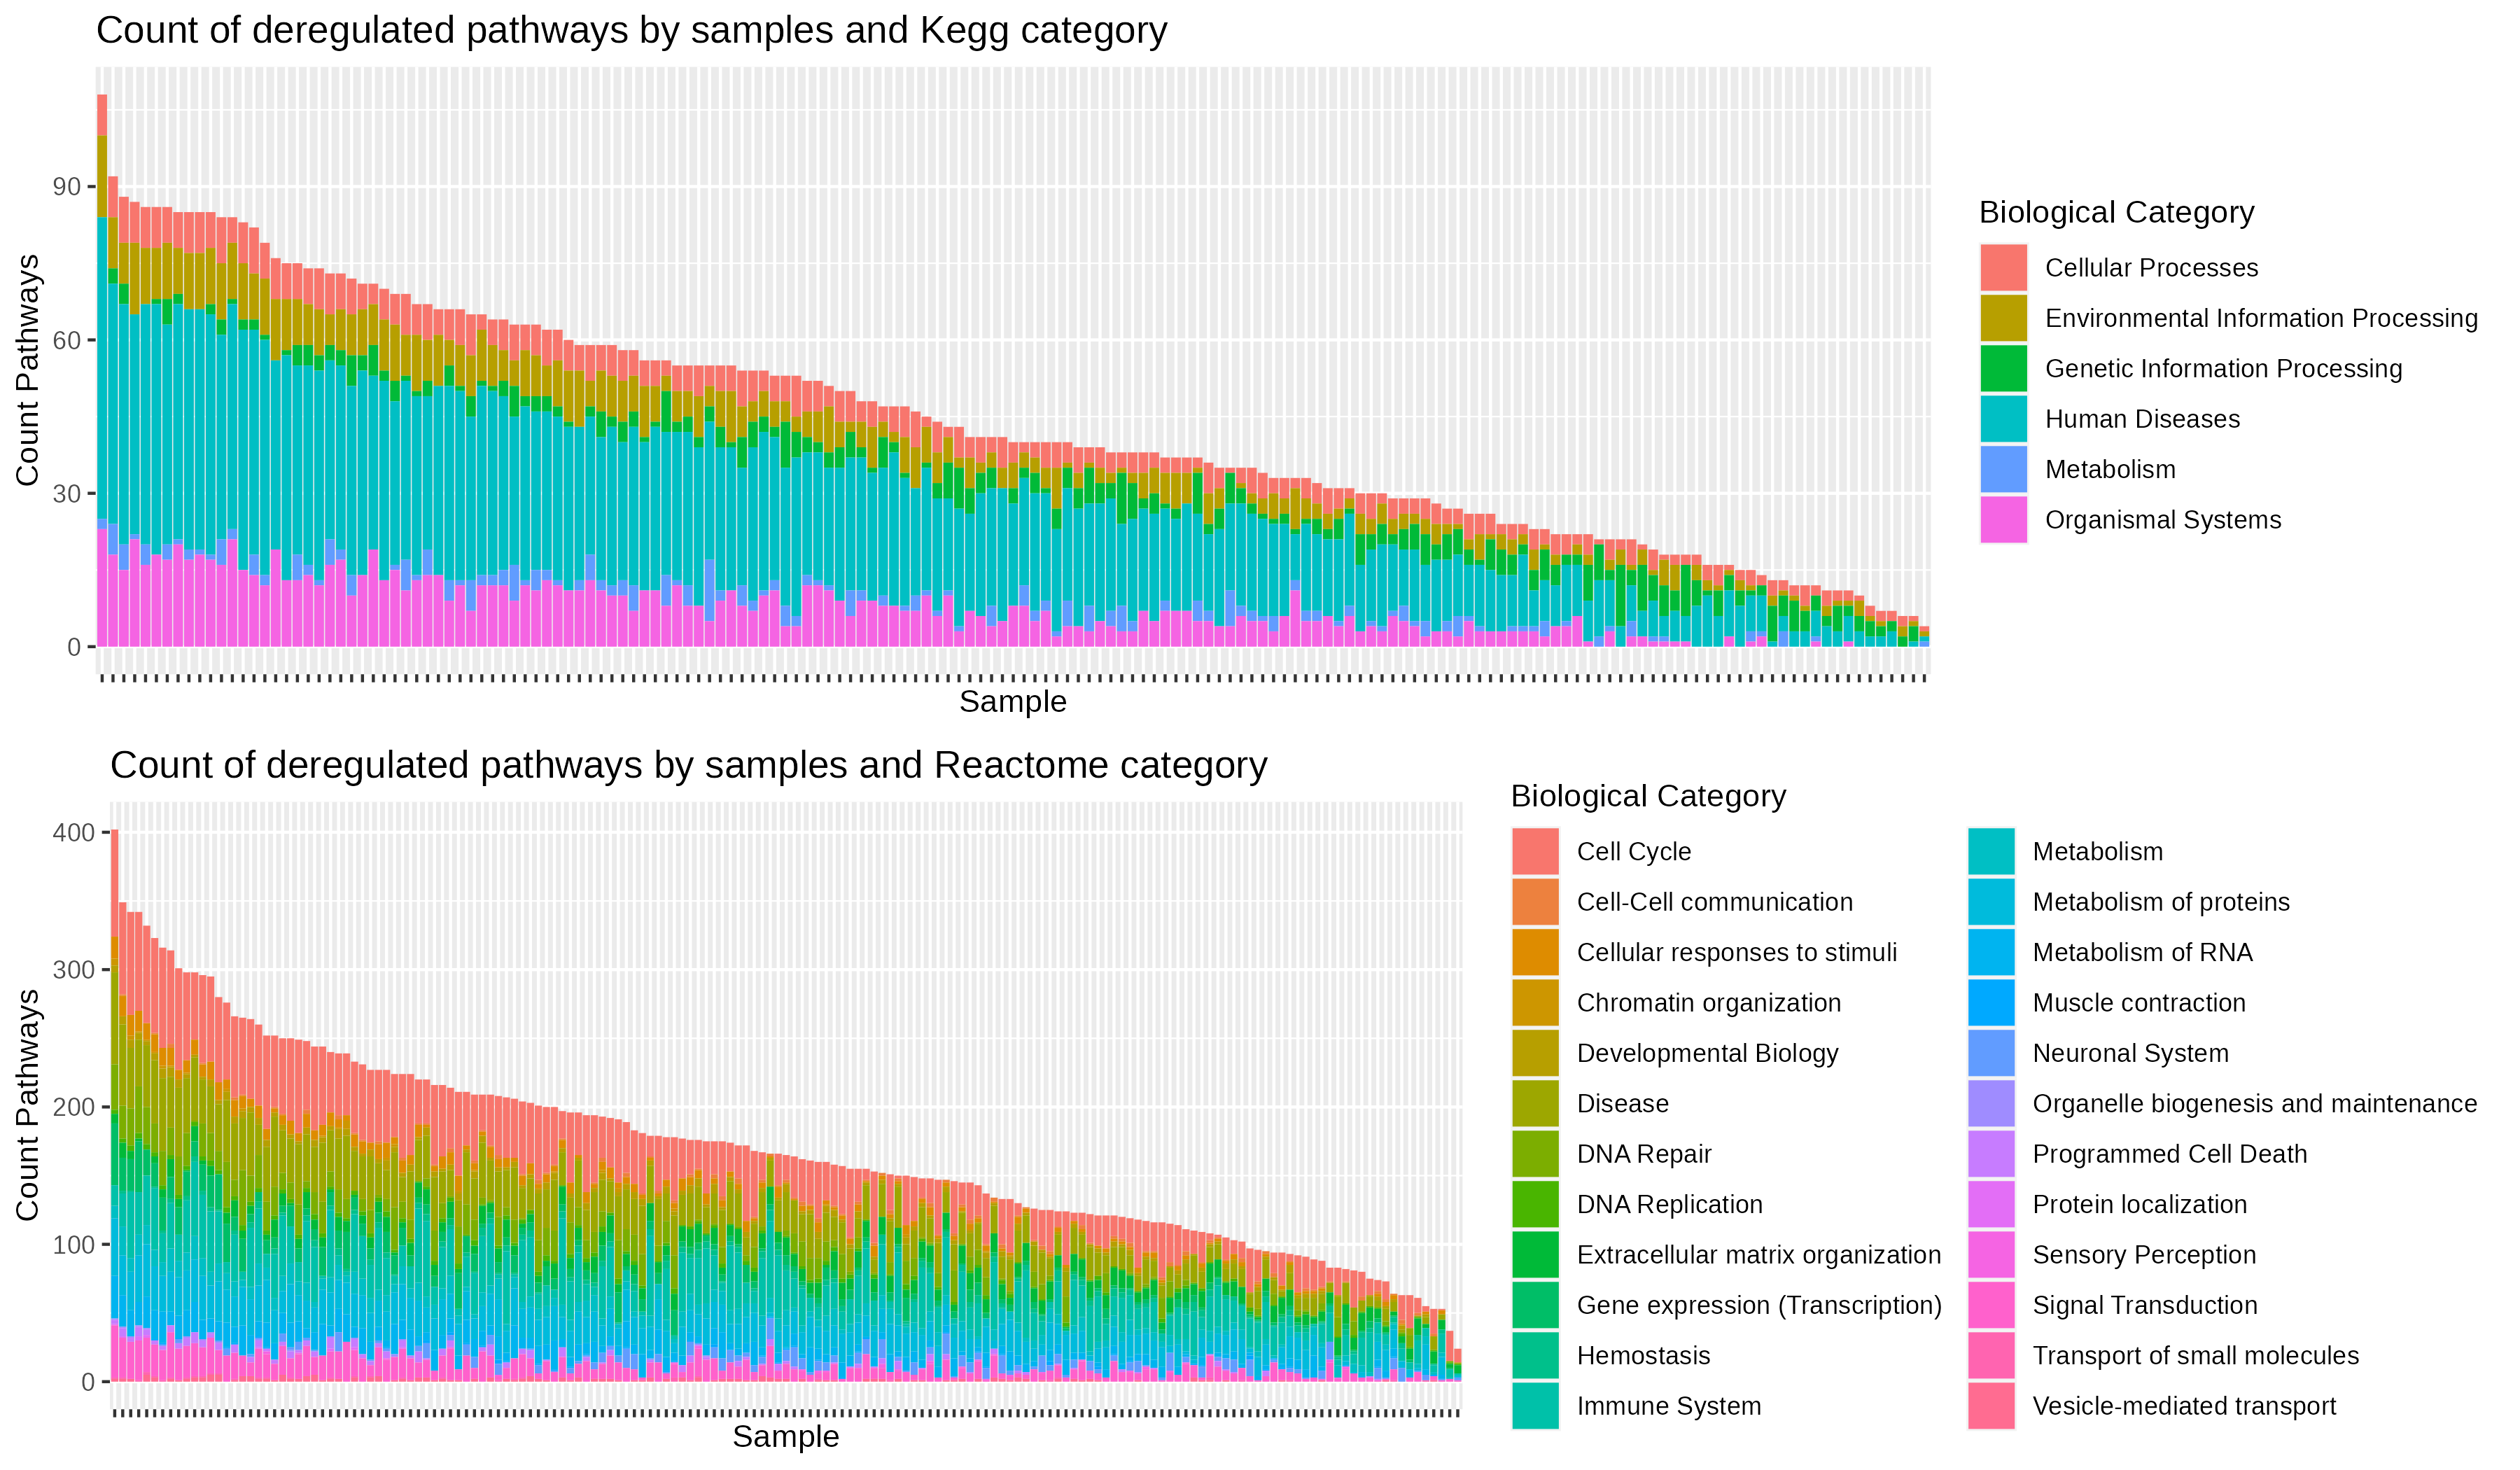
\includegraphics[width=0.8\textwidth]{img/barplot-categ-tcga}
        \caption{
            Number of deregulated pathways per category and per sample in the \acrshort{tcga} dataset.
            Sample names are not displayed to avoid overploting.
            Like the result with \acrshort{pdcl} samples, the \textit{Disease} is among the most deregulated categories in both \acrshort{kegg} and Reactome.
            While with \acrshort{pdcl}, Reactome pathways associated to the Cell-Cycle were predominantly deregualted in one sample, in \acrshort{tcga} the Cell-Cycle was greatly affected among all the samples.
        }
        \label{fig:barplot-categ-tcga}
    \end{center}
\end{figure}

Like for the \acrshort{pdcl} dataset, we investigated what were the most affected biological categories for each samples and show the results in figure \ref*{fig:barplot-categ-tcga}.
Same as in the \acrshort{pdcl}, the \textit{Disease} category is highly enriched in boh \acrshort{kegg} and Reactome.
However, more different Reactome categories are present in the results with \acrshort{tcga}.
In addition, while the \textit{Cell-Cycle} Reactome category was mostly observed affected in the \acrshort{pdcl} sample named \textit{4339-p21} (which was also the most affected sample), this category is greatly altered in all sample for \acrshort{tcga}.
\acrshort{tcga} results are also marked by an increased alteration of protein's metabolism across all the samples.

\subsubsection{Sample clustering by their deregulated categories}

For each sample, we divided the number of pathways deregulated in a category by the total number of pathways associated with this category in the \acrshort{gmt} file.
We used the vector of values generated to perform clustering of the samples using the K-Means algorithm with 3 clusters.
The number of clusters was chosen graphically by studying the correlation of each category to the principal components and with the coordinates of the samples in the new space.
Clustering results are shown in figure \ref*{fig:cluster-plot}.
Results are displayed in two dimensions using the first 2 components of a \acrshort{pca} on the same data used for clustering.
There is a better delimitation of the cluster using \acrshort{kegg} categories than with Reactome in two dimensions for both datasets.
There is some overlap between the clusters defined using Reactome categories in both datasets.
Reactome has more categories defined and used for clustering than \acrshort{kegg}, thus filtering out some categories that are not relevant for a study may facilitate the interpretation of the results.

\begin{figure}
    \begin{center}
        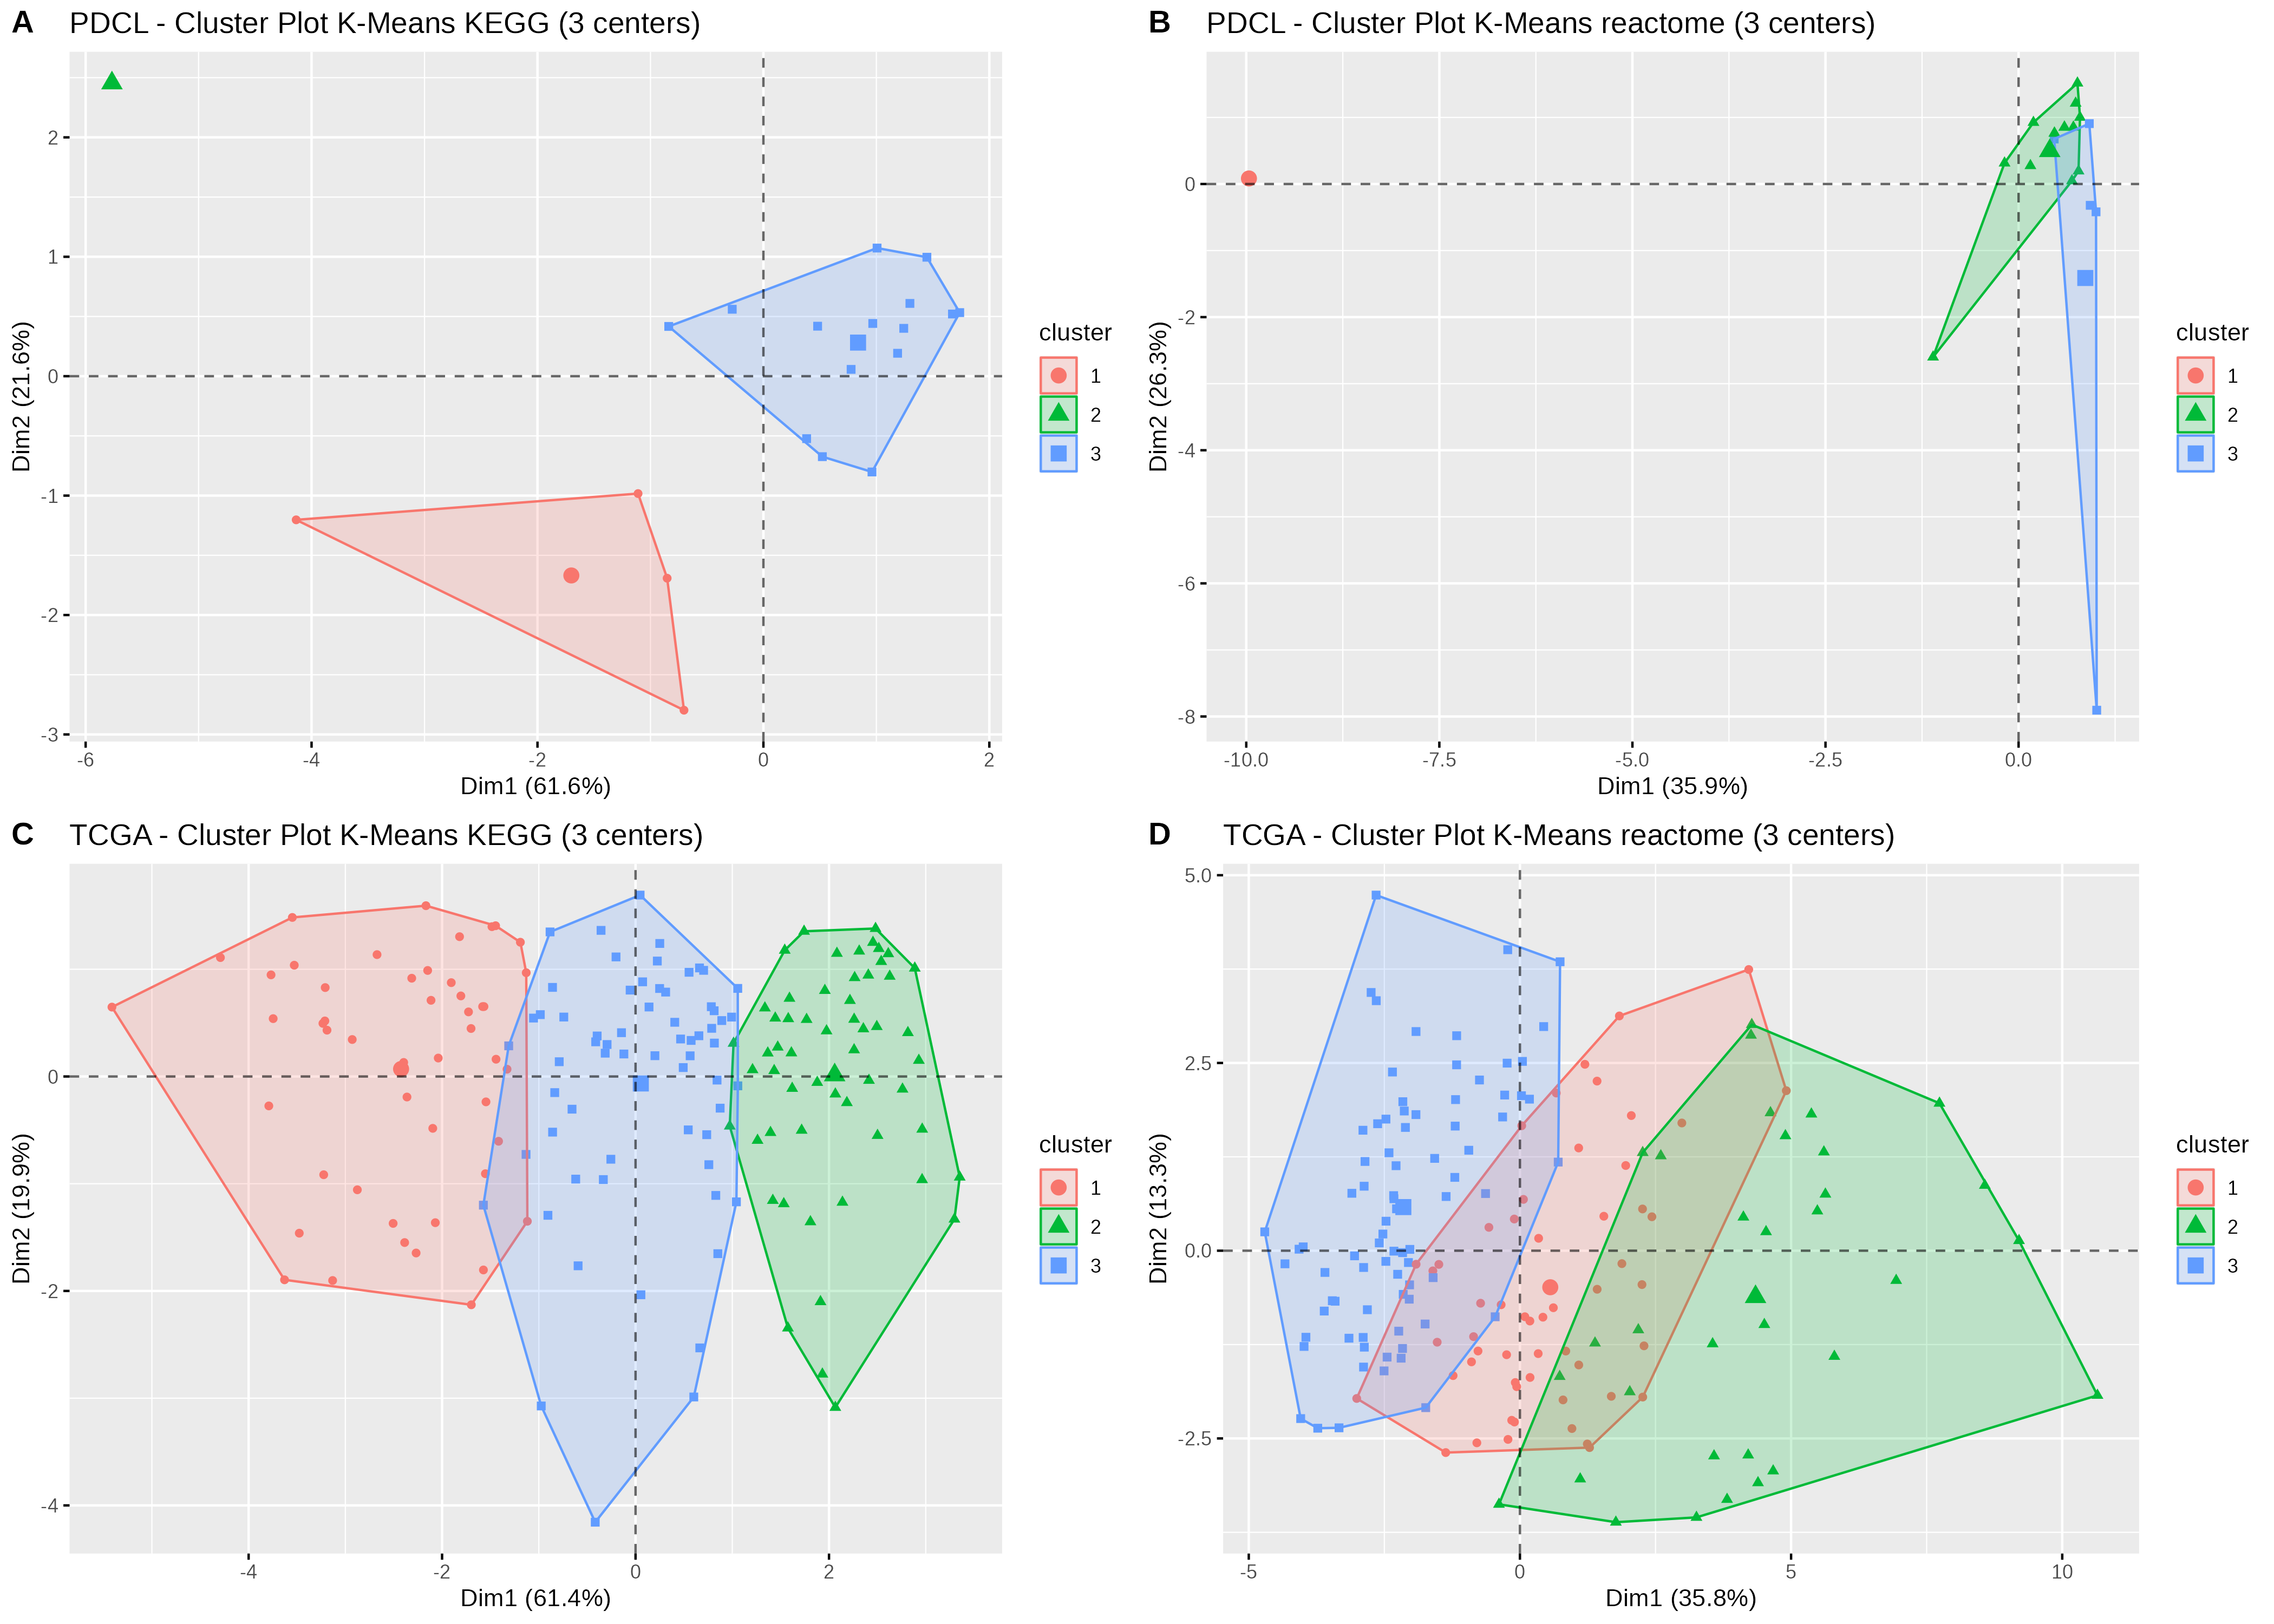
\includegraphics[width=\textwidth]{img/plot_cluster}
        \caption{
            Clustering of (A-B) \acrshort{pdcl} and (C-D) \acrshort{tcga} samples using the percentage of deregulation per biological categories.
            Results are shown with \acrshort{kegg} and Reactome categories.
            To generate a vector of values for each sample, we divided the number of pathways found significantly enriched for a category by the number of total pathways in this category present in the \acrshort{gmt} file.
            Clustering was done using the K-Means method with 3 clusters.
            In A (\acrshort{pdcl} samples with \acrshort{kegg} categories), cluster 1 seems to contain samples pathways that are associated with the \textit{Organismal Systems/Environmental Information processing/Human Diseases}, cluster 2 contains samples with deregulated pathways associated with \textit{Metabolism/Cellular Processes/Genetic Information Processing}, and the cluster 3 contains samples with few deregulated pathways.
            In B (\acrshort{pdcl} with Reactome categories), cluster 1 contains samples with deregulated pathways associated with \textit{Cell-Cycle/DNA replication and repair/Gene expression/Signal Transduction/Immune System}, cluster 2 with mainly \textit{Metabolism}, and the cluster 3 with mainly \textit{\acrshort{ecm}/Neuronal System/Disease/Transport of small molecules}.
            In C (\acrshort{tcga} with \acrshort{kegg}), the cluster 1 contains samples with deregulated pathways mainly associated with \textit{Environmental Information Processing/Organismal Systems/Human Diseases/Cellular Processes}, the cluster 2 with \textit{Metabolism}, and the cluster 3 with \textit{Genetic Information Processing}.
            In D (\acrshort{tcga} with Reactome), cluster 1 contains samples with deregulated pathways mainly associated with \textit{Immune System/Programmed Cell Death/Metabolism/Signal Transduction/Cellular Response to Stimuli/Vesicle-mediated transport}, the cluster 2 with \textit{Cell-Cycle/DNA replication/DNA repair/Chromatin organization/Gene Expression (Transcription)}, and the cluster 3 with \textit{\acrlong{ecm} Organisation/Cell-Cell communication/Hemostasis}.
        }
        \label{fig:cluster-plot}
    \end{center}
\end{figure}

Clustering of \acrshort{tcga} samples seems to separate samples with deregulated functions involved in the \textit{Metabolism}, genetic processing like \textit{DNA replication/repair} and processes linked to the extracellular environment like \textit{\acrshort{ecm} organization} or \textit{Environmental information processing} across both pathway databases.
A similar pattern is observed with \acrshort{pdcl} sample clustering with Reactome, although it seems that \textit{Metabolism} is less associated with deregulation than other categories (such as \textit{Signal Processing}).
Interestingly, when using \acrshort{kegg} categories to cluster \acrshort{pdcl} samples, one cluster seems to group samples that have less deregulated pathways and the \acrshort{pca} tend to separate samples mainly on this criterion.
